% Created 2020-02-17 Mo 14:40
% Intended LaTeX compiler: xelatex
\documentclass[aspectratio=169, 16pt]{beamer}
\usepackage{graphicx}
\usepackage{grffile}
\usepackage{longtable}
\usepackage{wrapfig}
\usepackage{rotating}
\usepackage[normalem]{ulem}
\usepackage{amsmath}
\usepackage{textcomp}
\usepackage{amssymb}
\usepackage{capt-of}
\usepackage{hyperref}
\usepackage{xcolor}
\usepackage{physics}
\usepackage{siunitx}
\usepackage{booktabs}
\usepackage[babel]{microtype}
\author{Michael Eliachevitch}
\date{\today}
\title{Weekly report}
\subtitle{BAMM! Meeting -- My train is 30 minutes late, so I'll be at the Bonn Hbf at 10:45. Slides are WIP in the train.}
\usepackage{templates/metropolisbonn}
\usepackage{hepnames, hepparticles}
\usepackage{tikz} \usetikzlibrary{positioning}
\newcommand{\PDmstar}{\HepParticle{D}{}{\left(*\right)}}
\newcommand{\rdstar}{R\left(\PDmstar\right)}
\institute{Physikalisches Institut --- Rheinische Friedrich-Wilhelms-Universität Bonn}
\hypersetup{colorlinks, urlcolor=bonnblue}
\lstset{keywordstyle=\bfseries\color{bonnblue}, commentstyle=\itshape\color{bonnunigrau}, identifierstyle=\color{bonntextgrau}, stringstyle=\color{bonnyellow}}
\hypersetup{
 pdfauthor={Michael Eliachevitch},
 pdftitle={Weekly report},
 pdfkeywords={},
 pdfsubject={},
 pdfcreator={Emacs 28.0.50 (Org mode 9.3.4)}, 
 pdflang={English}}
\begin{document}

\maketitle
\begin{frame}[label={sec:org3a79f7f},fragile]{Overview of things I did last week}
 \begin{itemize}
\item use histogramming functions from \texttt{TemplateFitter}
\item learn Dask and use it in my notebook
\item write luigi task for pickling steering files and sending to grid
\end{itemize}
\end{frame}

\begin{frame}[label={sec:org96999f6},fragile]{Use \texttt{TemplateFitter} histogram classes and plot styles}
 \begin{itemize}
\item still only reconstructing \(B \rightarrow D (\rightarrow K\pi\pi) \ell \nu_{\ell}\)
\item \texttt{isSignal} for B decays already fixed, but not in plots
\end{itemize}
\begin{columns}
\begin{column}{0.33\columnwidth}
\(M_{D^+}\)
\begin{center}
\includegraphics[width=.9\linewidth]{./figures/M_D.pdf}
\end{center}
\end{column}
\begin{column}{0.33\columnwidth}
\(M_{bc}\)
\begin{center}
\includegraphics[width=.9\linewidth]{./figures/B_Mbc.pdf}
\end{center}
\end{column}
\begin{column}{0.33\columnwidth}
\(\Delta E\)
\begin{center}
\includegraphics[width=.9\linewidth]{./figures/B_deltaE.pdf}
\end{center}
\end{column}
\end{columns}
\end{frame}
\begin{frame}[label={sec:org3365595},fragile]{Dask}
 \begin{description}
\item[{pandas}] useful for exploration, but requires all data in memory\\
workaround: do cuts, save to disk and read only required branches into memory
\item[{root}] iterates over data on disk, recently implemented its own \texttt{RDataFrames}
\item[{\href{https://dask.org/}{dask}}] \texttt{daskarray} \& \texttt{daskframe}: \alert{blocked} alternatives for \texttt{np.array} \& \texttt{pd.DataFrame}
\begin{itemize}
\item delays all calculations until the final \texttt{.compute()} is called
\item delayed calculations make up graph (similar to \texttt{luigi}, \texttt{tensorflow}, \texttt{basf2.add\_module})
\item loads only blocks that it currently needs into memory
\item dask scheduler parallelizes computations and manages memory
\item \href{https://stackoverflow.com/questions/60189433/how-to-avoid-too-many-open-files-error-when-using-uproot-daskframes-to-create/60191127\#60191127}{stackoverflow} on reading many root files into daskframe
\end{itemize}
\end{description}
\end{frame}

\begin{frame}[label={sec:org5b4ee6c},fragile]{Example dask computation graphs}
 \begin{columns}
\begin{column}{0.5\columnwidth}
\lstset{language=Python,label= ,caption= ,captionpos=b,numbers=none,basicstyle=\tiny\ttfamily, xleftmargin=-5pt}
\begin{lstlisting}
D_dd = daskframe_from_rootfiles(
    Dplus_ntupels[0:5], key="ntuple")
D_dd.isSignal.sum().visualize()
\end{lstlisting}
\begin{center}
\includegraphics[width=.55\textwidth]{./figures/dask_graph_sum.pdf}
\end{center}
\end{column}
\begin{column}{0.5\columnwidth}
\lstset{language=Python,label= ,caption= ,captionpos=b,numbers=none,basicstyle=\tiny\ttfamily, xleftmargin=-5pt}
\begin{lstlisting}
h, bins = da.histogram(
    D_dd.M, bins=np.linspace(1.8, 1.9, 10))
h.visualize()
\end{lstlisting}
\begin{center}
\includegraphics[width=.45\textwidth]{./figures/dask_graph_hist.pdf}
\end{center}
\end{column}
\end{columns}
\end{frame}

\begin{frame}[label={sec:orgdae7e94}]{How to I send grid jobs without needing the python packages installed there}
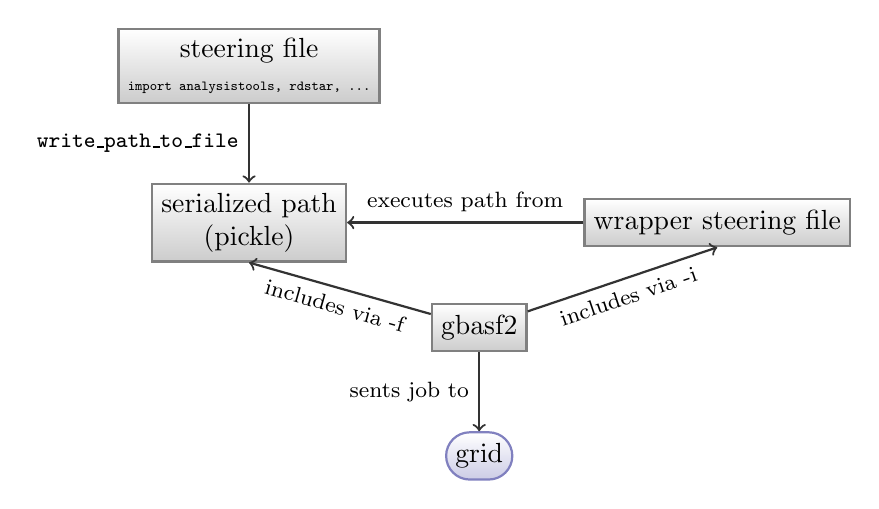
\begin{tikzpicture}[
align=center,
    mybox/.style={
    rectangle,minimum size=6mm,
    thick,draw=black!50,
    top color=white,bottom color=black!20},
    gridbox/.style={
    rectangle,minimum size=6mm,rounded corners=3mm,
    thick,draw=black!50!blue!50,
    top color=white,bottom color=blue!50!black!20,
    }
    ]

    \node [mybox] (steeringfile) {steering file\\ \ttfamily{\tiny import
    analysistools, rdstar, \ldots}};
    \node [mybox, below=of steeringfile] (pickle) {serialized path\\(pickle)};
    \node [mybox, right=3cm of pickle] (wrapper) {wrapper steering file};
    \node [mybox, below left=1cm of wrapper] (gbasf2) {gbasf2};
    \node [gridbox, below=of gbasf2] (grid) {grid};
    \draw [->, thick, draw=black!80] (steeringfile) -- (pickle) node
    [font=\footnotesize\ttfamily, midway, left] {write\_path\_to\_file};
    \draw [->, thick, draw=black!80] (wrapper) -- (pickle) node
    [font=\footnotesize, midway, above] {executes path from};
    \draw [->, thick, draw=black!80] (gbasf2) -- (wrapper.south) node
    [font=\footnotesize, midway, sloped, below] {includes via -i};
    \draw [->, thick, draw=black!80] (gbasf2) -- (pickle.south) node
    [font=\footnotesize, midway, sloped, below] {includes via -f};
    \draw [->, thick, draw=black!80] (gbasf2) -- (grid) node
    [font=\footnotesize, midway, left] {sents job to};
\end{tikzpicture}
\end{frame}
\end{document}